\chapter{Introduction}
\label{chapter:introduction}

Twenty years after its birth, the Web has become one of the defining
technological innovations that knows no geographical, political, or
ideological boundaries. The world wide platform built on top of the
physical Internet is deeply integrated into our daily lives. This
powerful tool that was built on egalitarian principles is now taken
for granted, just like old innovations such as
electricity. \cite{berners2010long}

In parallel with the rapid growth of the Web, mobile phones have
evolved from briefcase-sized ``portable'' telephony devices into
modern pocket-sized computers. The mobile revolution has already
changed the world as we see it, and more people have access to the Web
from a mobile device than from an Internet-connected desktop
computer. \cite{fling2009mobile}

The Web is not constrained into (desktop and laptop) computers and
mobile phones, though. Tablets, TVs, ebook readers, watches, and even
household appliances are connecting to the Internet and have web
browsers. For the first time in history, we have a truly ubiquitous
digital medium. \cite{fling2009mobile}

Universal accessibility and openness are the keys to being the
ubiquitous information platform of the digital age
\cite{berners2010long}. Now the Web is closer in accomplishing its
original principles in equality and universality; anyone can access
this vast source of open information from anywhere, with any
device. All you need is a web browser that supports the open standards
of the Web.

\begin{quotation}
  \noindent \textit{The goal of the Web is to serve humanity.}
  \begin{flushright}
    -- Tim Berners-Lee \cite{berners2010long}
  \end{flushright}
\end{quotation}

Being the universal digital medium, mobile devices has some unique
characteristics that other mass media lack. Mobile is personal,
always-on, always-carried medium with a built-in payment
channel. Mobile is in your pocket at the moment you have your creative
impulse. \cite{fling2009mobile}

These characteristics have made mobile device applications a
multibillion-dollar business. Five years after Apple published its
game-changing iPhone and the App Store, touch screen mobile phones and
tablets from different device manufacturers have spread all over the
world. \cite{cortimiglia2011mobile, charland2011mobile,
  fling2009mobile}

However, this proliferation of mobile devices and platforms has raised
a serious issue for application developers: fragmentation. Not only
are there multiple target platforms, but even within the platforms
there are different versions with different feature sets, not to
mention different devices with varying
capabilities. \cite{charland2011mobile}

\begin{table}
  \begin{tabular}{ l | l }
    \textbf{Mobile OS Type} & \textbf{Skill Set Required} \\
    \hline
    Apple iOS & C, Objective C \\
    Google Android & Java (Harmony flavored, Dalvik VM) \\
    RIM BlackBerry & Java (J2ME flavored) \\
    Symbian & C, C++, Python, HTML/CSS/JS \\
    Windows Mobile & .NET \\
    Windows 7 Phone & .NET \\
    HP Palm webOS & HTML/CSS/JS \\
    MeeGo & C, C++, HTML/CSS/JS \\
    Samsung bada & C++
  \end{tabular}
  \label{table:native-skills}
  \caption{Required developer skill sets for different mobile
    platforms according to \cite{charland2011mobile}}
\end{table}

Table~1.1\tablerefs shows the required developer skill sets for
different platforms. As we see, each platform has its own programming
language and \abbr{SDK}. A lot of knowledge and resources are needed
to provide cross-platform applications for these platforms. Making
several independent applications with the native tools is also very
expensive, and adding features or just maintaining all these different
applications becomes costly. \cite{charland2011mobile}

Some developers are forced to make compromises due to resourcing or
budgeting, and build their applications only for one platform. This
might be fine for independent developers, but a lot of potential
customers or users are left out of these walled gardens. Big
corporations or public organizations cannot afford leaving out large
shares of the mobile market (see smartphone sales by operating system
in Figure~\ref{figure:market-share.png}). \cite{berners2010long}

\begin{figure}[h!]
  \begin{center}
    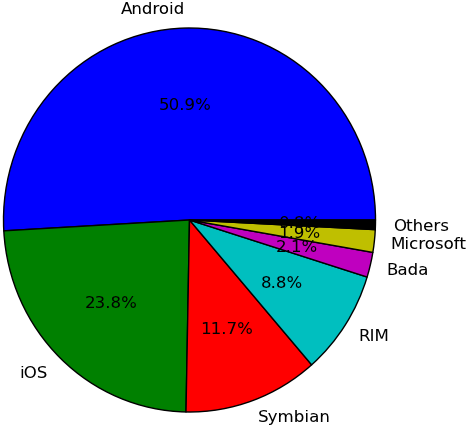
\includegraphics[width=0.6\textwidth]{images/market-share.png}
    \caption{Worldwide Smartphone sales by operating systems in 4Q
      2011 according to
      \url{http://www.gartner.com/it/page.jsp?id=1924314}}
    \label{figure:market-share.png}
  \end{center}
\end{figure}

Being cross-platform is essential in today's mobile market. And if the
required skills and resources for the native tools are not present,
other options have to be considered. All mobile devices have a web
browser, and the Web is becoming the universal application
platform. \cite{taivalsaari2011web, mikkonen2011apps}

In the 20 years of its lifetime, the Web has evolved from a simple
system for sharing documents into a massively popular, world wide
application and information distribution environment
\cite{taivalsaari2011web}. During the so-called Web 2.0 revolution,
the Web grew into a platform for interactive applications with the
help of technologies like \abbr{Ajax} \cite{garrett2005ajax}.

The Web is not without its problems, however. The viral spreading of
mobile phones has raised the need for a feature-rich technology stack
for building scalable applications that can handle the whole spectrum
of devices, screen sizes, and form factors that are used to access the
Internet. This is the need that \abbr{HTML5} with all the related
tools and \abbr{APIs} have promised to solve.

Performance is the foundation of a great user experience
\cite{charland2011mobile}. By performance, I mean the speed of
downloading, initializing and using an application as perceived by the
user as well as the responsiveness and smoothness of the user
interface influencing the overall user experience.

Native tools have been carefully optimized to provide the best
possible performance and responsiveness, and web applications are
often unfavorably compared to them. In the end, however, the received
savings in development time, deployment, cost-efficiency, and
cross-platform support can often outweigh the possible
compromises. \cite{charland2011mobile, fling2009mobile}

In this work I look at the performance of \abbr{HTML5} as a
cross-platform application platform for different device
form-factors. To study the performance, I built a real-world HTML5
application and a JavaScript library and fine-tuned the performance to
get the best possible user experience. I then asses these
optimizations and the compromises that had to be made.

\section{Research Questions}
\label{section:research-questions}

Knowing the reasons and motivation for cross-platform HTML5 and the
importance of application performance and responsiveness:

\begin{itemize}
\item \textbf{RQ1}: \textit{What are the main problem areas in mobile
  web development?}

  Mobile web development is a large problem area, and dealing with
  relatively new technologies and large amounts of devices, finding
  the main problems is crucial for this work.

\item \textbf{RQ2}: \textit{Do HTML5 and related specifications solve
  these problems?}

  There are a lot of new specifications and \abbr{API}s for web
  development. Do these specifications solve the problems identified
  in answering RQ1?

\item \textbf{RQ3}: \textit{What other practical means do we have to
  solve these problems?}

  Not all problems can be solved with specifications and new standard
  \abbr{API}s. What other practical means and techniques can be used
  to solve the problems identified in RQ1?

\end{itemize}

I introduce the HTML5 specification and other related standards in a
generic way, but the practical research is constrained into using the
new \abbr{API}s in a real-world mobile application. Thus not all APIs
are applicable or needed, but the ones used are deployed for real end
users and examined in the current browser implementations. Being a
large topic, this work focuses especially on the performance aspect of
the latest APIs and their current implementations to get a good
overview of the application of the specifications in a real-world
scenario.

\section{Structure of This Work}
\label{section:structure-of-this-work}

In Chapter~\ref{chapter:html5} and
Chapter~\ref{chapter:other-related-specifications} I introduce HTML5
and related specifications and \abbr{API}s for modern web
development. In Chapter~\ref{chapter:tools-and-techniques} I present
some of the latest tools, frameworks and libraries for building mobile
web applications.

In Chapter~\ref{chapter:use-case} I introduce the practical part of
this work and its requirements, and in
Chapter~\ref{chapter:implementation} I present the implementation
details and results of the practical research. In
Chapter~\ref{chapter:conclusions} I sum up the work and discus further
work ideas.
